\chapter{Conclusions}
\graphicspath{{conclusions/figs}}

A brief introduction

\section{Research Conclusions}
%\subsubsection{\nameref{chapter:continuous_compost_bomb}}

In \cref{chapter:continuous_compost_bomb} I investigated the the effect of adding a vertical spatial dimension to the compost bomb instability.
The purpose of this was twofold. 
Firstly, I was interested to see if the instability still existed in a more realistic model.
Secondly, I wanded to know if certain wildfires could be caused by biogeochemical heating and in order to do this more realistic physics was desirable.

\todo[inline]{Expand on Siberian wildfires. add a para?}

In order to investigate this, I created a partial differential equation model of soil temperature which included biogeochemical heating. I made the assumption
that soil carbon could be viewed as being time invariant, which placed the model into the `compost bomb limit' of~\cite{Luke2011}. This came at the cost of preventing
R-tipping so the potential for B-tipping was investigated. Furthermore the effect of a large seasonal cycle in atmospheric temperatures on the soil was investigated.

It was shown that for sufficently large atmospheric temperatures the model had no steady state. This meant that the soil temperatures had diverged and that a compost bomb
had occured. If, as in the real world, soil carbon were allowed to evolve dynamically then the amount of soil carbon would decrease which would prevent the soil temperatures from diverging;
instead they would simply reach a large value.

It was also shown that a sufficently large seasonal cycle --- which could be realised by a summer heat wave --- would be enough to trigger a compost bomb.
Furthermore, the size of the seasonal cycle was not dissimilar to the seasonal cycles observed in parts of Siberia (as shown in \cref{fig:seasonal_cycle_maps}).
This can be seen as evidence that Siberian wildfires may be caused, in part, by biogeochemical heating. 

\begin{figure}
  \centering
  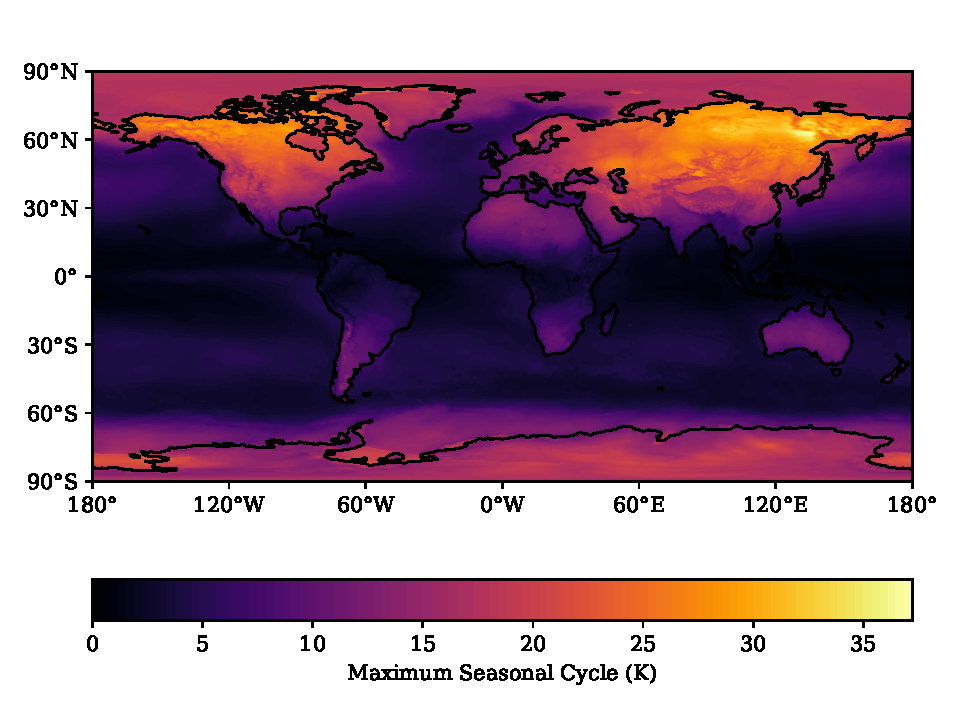
\includegraphics[width=\textwidth,keepaspectratio]{seasonal_cycles}
  \caption[Map of Seasonal Cycles]{The largest observed seaonsonal cycle in the ERA5 reanalysis \parencite{Hersbach2020} over the period 1940--2022.
    The magnitude of the seasonal cycle is defined as half the difference between the maximum and minimum monthy averaged \SI{2.0}{\meter} air temperatures.}
  \label{fig:seasonal_cycle_maps}
\end{figure}

\todo[inline]{misc crit of model}

Due to the approximation that soil carbon was constant in time, the compost bomb instability became an example of B-tipping rather than R-tipping. It does not necessarily
follow that the system would experience R-tipping if this approximation was relaxed. However, it is reasonable to assume that the vertical diffusion of heat would not be a barrier to
R-tipping, as long as the atmospheric temperatures were raised rapidly compared to the soil carbon timescale, due to the significant timescale separation between the soil thermal and
carbon timescales \parencite{Luke2011}.

The approximation that soil carbon is constant is accurate over the timescales of a year, given the decadal turnover time of soil carbon \parencite{Varney2020}.
It follows therefore, that there can be good confidence about the results to do with the seaonal cycle. However, the applicability to the phenomenon of wildfires is more doubtful.
This is because it may be better to view a hot summer period as a more temporally compact perturbation to atmospheric temperatures, rather than an amplified sinusoid. This case has
since been studied by~\cite{OSullivan2023} for the model of~\cite{Luke2011}. They also found for realistic Siberian summer temperatures compost bombs were possible. 

To summarise, in \cref{chapter:continuous_compost_bomb} I managed to show that adding in the vertical diffusion of heat does not suppress the compost bomb. This therefore increases the confidence
that the effect is real. Furthermore I also showed that a hot summer, as modeled by a large seasonal cycle of temperature, could cause compost bombs, which has applications to the
problem of Siberian wildfires.
\section{Outlook}

A graceful landing?